% Created 2022-06-03 Fri 15:39
% Intended LaTeX compiler: xelatex
\documentclass[aspectratio=1610,hyperref={colorlinks,unicode,linkcolor=blue,anchorcolor=blue,citecolor=blue,filecolor=black,urlcolor=blue}]{beamer}
\usepackage{graphicx}
\usepackage{grffile}
\usepackage{longtable}
\usepackage{booktabs}
\usepackage{wrapfig}
\usepackage{rotating}
\usepackage[normalem]{ulem}
\usepackage{amsmath}
\usepackage{textcomp}
\usepackage{amssymb}
\usepackage{capt-of}
\usepackage[colorlinks,unicode,linkcolor=blue,anchorcolor=blue,citecolor=blue,filecolor=black,urlcolor=blue]{hyperref}
\usepackage{listings}
\usepackage{algorithm}
\usepackage{algpseudocode}
\usepackage[cache=false]{minted}
\usepackage{etoolbox}
\useoutertheme{infolines}
\setbeamertemplate{frametitle}{%
\usebeamerfont{frametitle}\insertframetitle\strut%
\vskip-0\baselineskip%
\leaders\vrule width .95\paperwidth\vskip1pt%
\vskip0pt%
\nointerlineskip
}

%% T for footer
\setbeamercolor{footlinecolor}{fg=cyan,bg=green}
\setbeamercolor{author in head/foot}{fg=blue}
\setbeamertemplate{footline}{%
\leavevmode%
\hbox{%
\begin{beamercolorbox}[wd=.26\paperwidth,ht=2.25ex,dp=1ex,left]{author in head/foot}%
\hspace*{2ex}\usebeamerfont{author in head/foot} Dept. CSE, UT Arlington
\end{beamercolorbox}%
\begin{beamercolorbox}[wd=.50\paperwidth,ht=2.25ex,dp=1ex,center]{author in head/foot}%
\usebeamerfont{title in head/foot}Scalable Modeling \& Imaging \& Learning Lab (SMILE)
\end{beamercolorbox}%
\begin{beamercolorbox}[wd=.24\paperwidth,ht=2.25ex,dp=1ex,right]{date in head/foot}%
\usebeamerfont{date in head/foot}
\insertshortdate{}\hspace*{1em}  % date
\insertframenumber/\inserttotalframenumber\hspace*{2ex}
\end{beamercolorbox}}%
\vskip0pt%
}
\usetheme{default}
\usefonttheme{serif}
\useinnertheme{circles}
\author{Ziniu Hu, Yuxiao Dong, Kuansan Wang, Yizhou Sun}
\date{Jun 03, 2022}
\title{Heterogeneous Graph Transformer}
\hypersetup{
 pdfauthor={Ziniu Hu, Yuxiao Dong, Kuansan Wang, Yizhou Sun},
 pdftitle={Heterogeneous Graph Transformer},
 pdfkeywords={},
 pdfsubject={},
 pdfcreator={Emacs 29.0.50 (Org mode 9.5)}, 
 pdflang={English}}
\usepackage{biblatex}
\addbibresource{/Users/Nasy/smile/pre/ref.bib}
\begin{document}

\maketitle
\begin{frame}{Outline}
\tableofcontents
\end{frame}


\section{Introduction}
\label{sec:orgef30a18}

\begin{frame}[label={sec:org61f9e7d}]{Introduction}
Heterogeneous Graph (HG) also known as heterogeneous information
networks (HIN).

A heterogeneous graph can represent as \(\mathcal{G} = (\mathcal{V},
\xi)\), where each node \(\mathcal{V}\), and each edge \(\xi\) has its own
type \(\Gamma_{v}\) and \(\Gamma_{e}\).  A heterogeneous graph have two
mapping function: \(\phi_{v}:V\rightarrow\Gamma_{v}\) for node to node
types, and \(\phi_{e}:\xi\rightarrow\Gamma_{e}\) for edge types.

\begin{center}
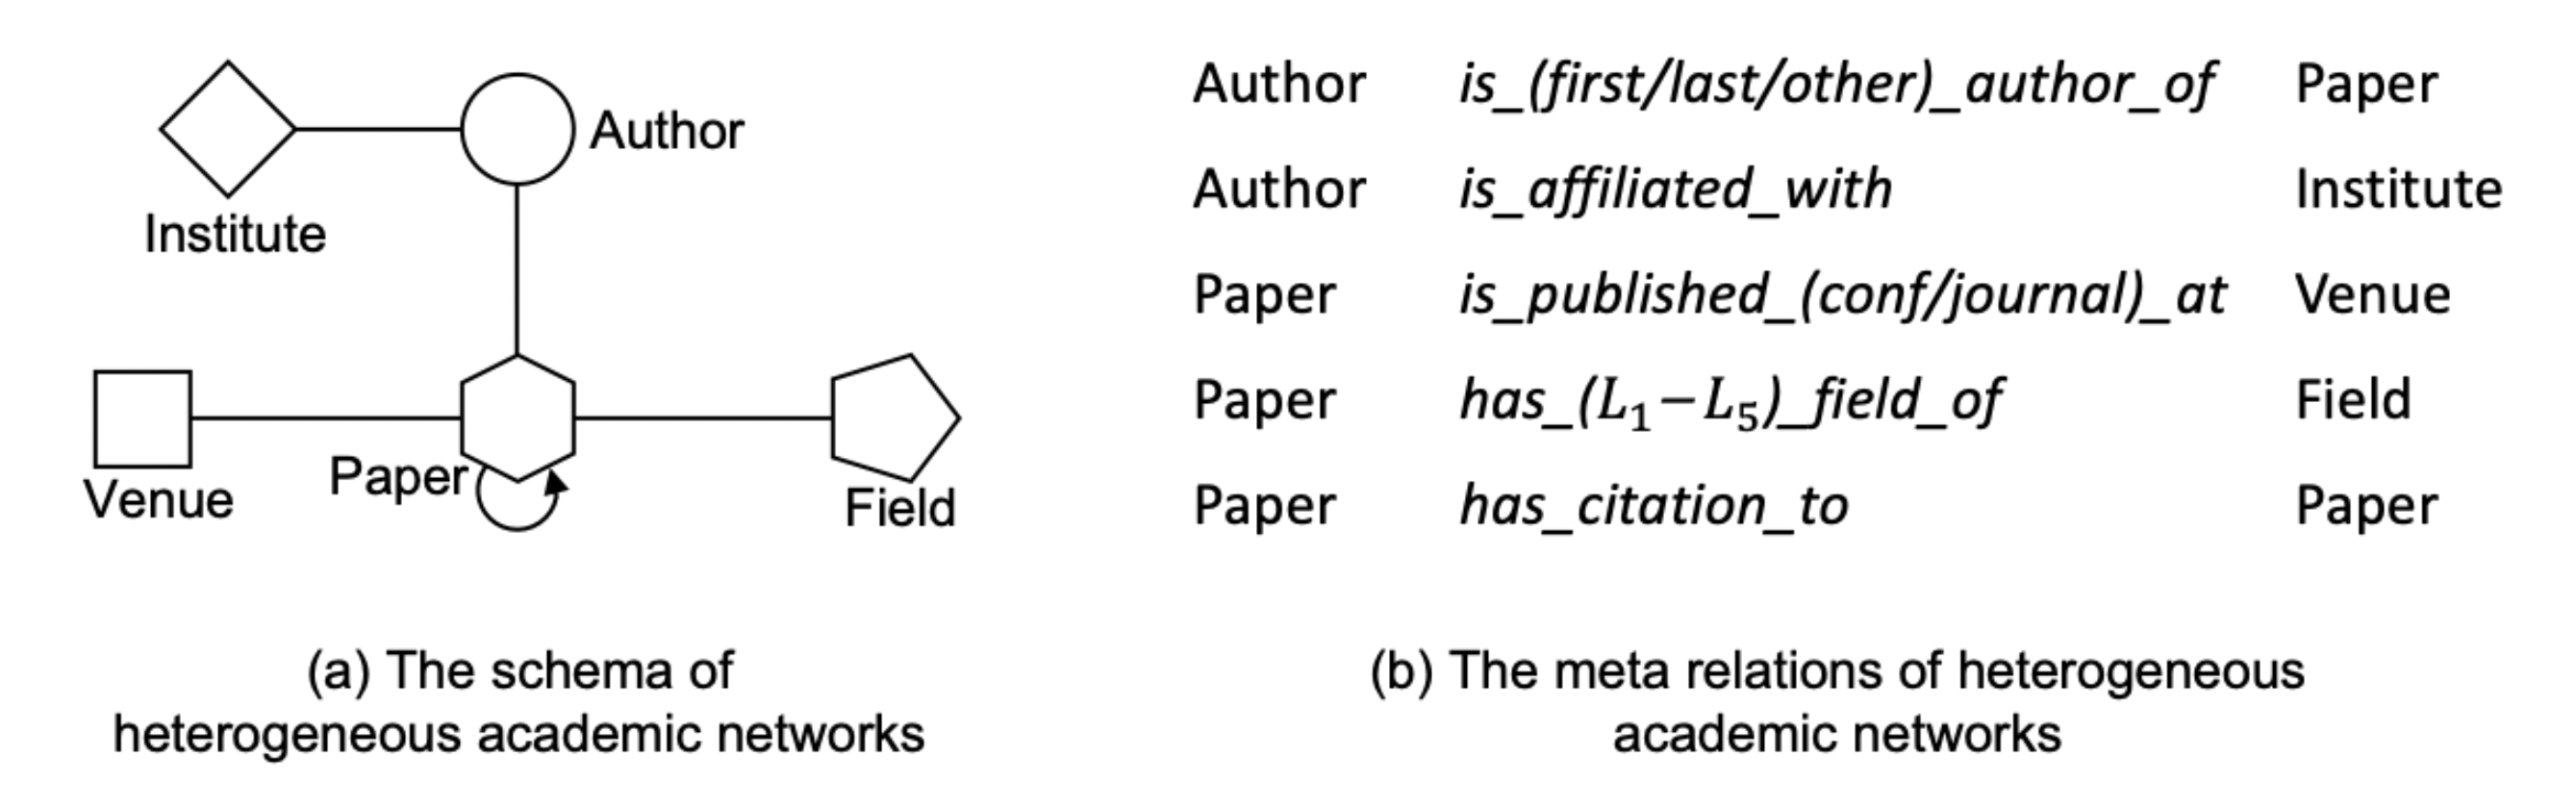
\includegraphics[width=.9\linewidth]{./p1.png}
\end{center}
\end{frame}

\begin{frame}[label={sec:orge14bd28}]{Problem}
\begin{itemize}
\item Meta-path need domain knowledge.
\item Different types of nodes/edges share features.
\item Different types of nodes/edges keep different non-shared weights
\item Ignore the dynamic of heterogeneous graph
\item Incapable of modeling Web-scale (large) heterogeneous graph
\end{itemize}
\end{frame}

\begin{frame}[label={sec:org4f4ef37}]{Heterogeneous graph transformer (HGT)}
\begin{itemize}
\item Node and edge type dependent attention mechanism.
\begin{itemize}
\item Not parameterizing each type of edges
\item use meta relation triplet \(e = (s, t)\), where \(s\) is source
node, \(t\) is target node
\end{itemize}
\item Relative temporal encoding (RTE) strategy for dynamic graph
\item HGSampling for Web-scale graph data.
\end{itemize}
\end{frame}

\section{Method}
\label{sec:orgb3ff278}

\begin{frame}[label={sec:org6006c9d}]{Symbols}
\begin{description}
\item[{Graph}] \(G = (\mathcal{V}, \mathcal{E}, \mathcal{A},
  \mathcal{R})\)
\item[{Node}] \(v \in \mathcal{V}\), also \(s,t\)
\item[{Edge}] \(e \in \mathcal{E}\)
\item[{Node Type}] \(\tau(v): \mathcal{V} \rightarrow
  \mathcal{A}\)
\item[{Edge Type}] \(\phi(e): \mathcal{E} \rightarrow
  \mathcal{R}\)
\item[{edge, source node, target node}] \(e = (s, t)\)
\item[{meta relation triplet}] \(<\tau(s),\phi(e),\tau(t)>\)
\end{description}
\end{frame}

\begin{frame}[label={sec:orgab989de}]{Method}
Use the \alert{meta-relations} fo heterogeneous graph to parameterize weight
matrices for heterogeneous mutual attention, message passing, and
propagation steps.

Three steps:

\begin{itemize}
\item Heterogeneous Mutual Attention
\begin{itemize}
\item input embedding of \(s_1,s_2,t\)
\item output attention matrix of \(\phi(e)\).
\end{itemize}
\item Heterogeneous Message Passing
\begin{itemize}
\item output message of \(\phi(e)\)
\end{itemize}
\item Target-Specific Aggregation
\end{itemize}
\end{frame}

\begin{frame}[label={sec:org4af6efc}]{Method}
\begin{center}
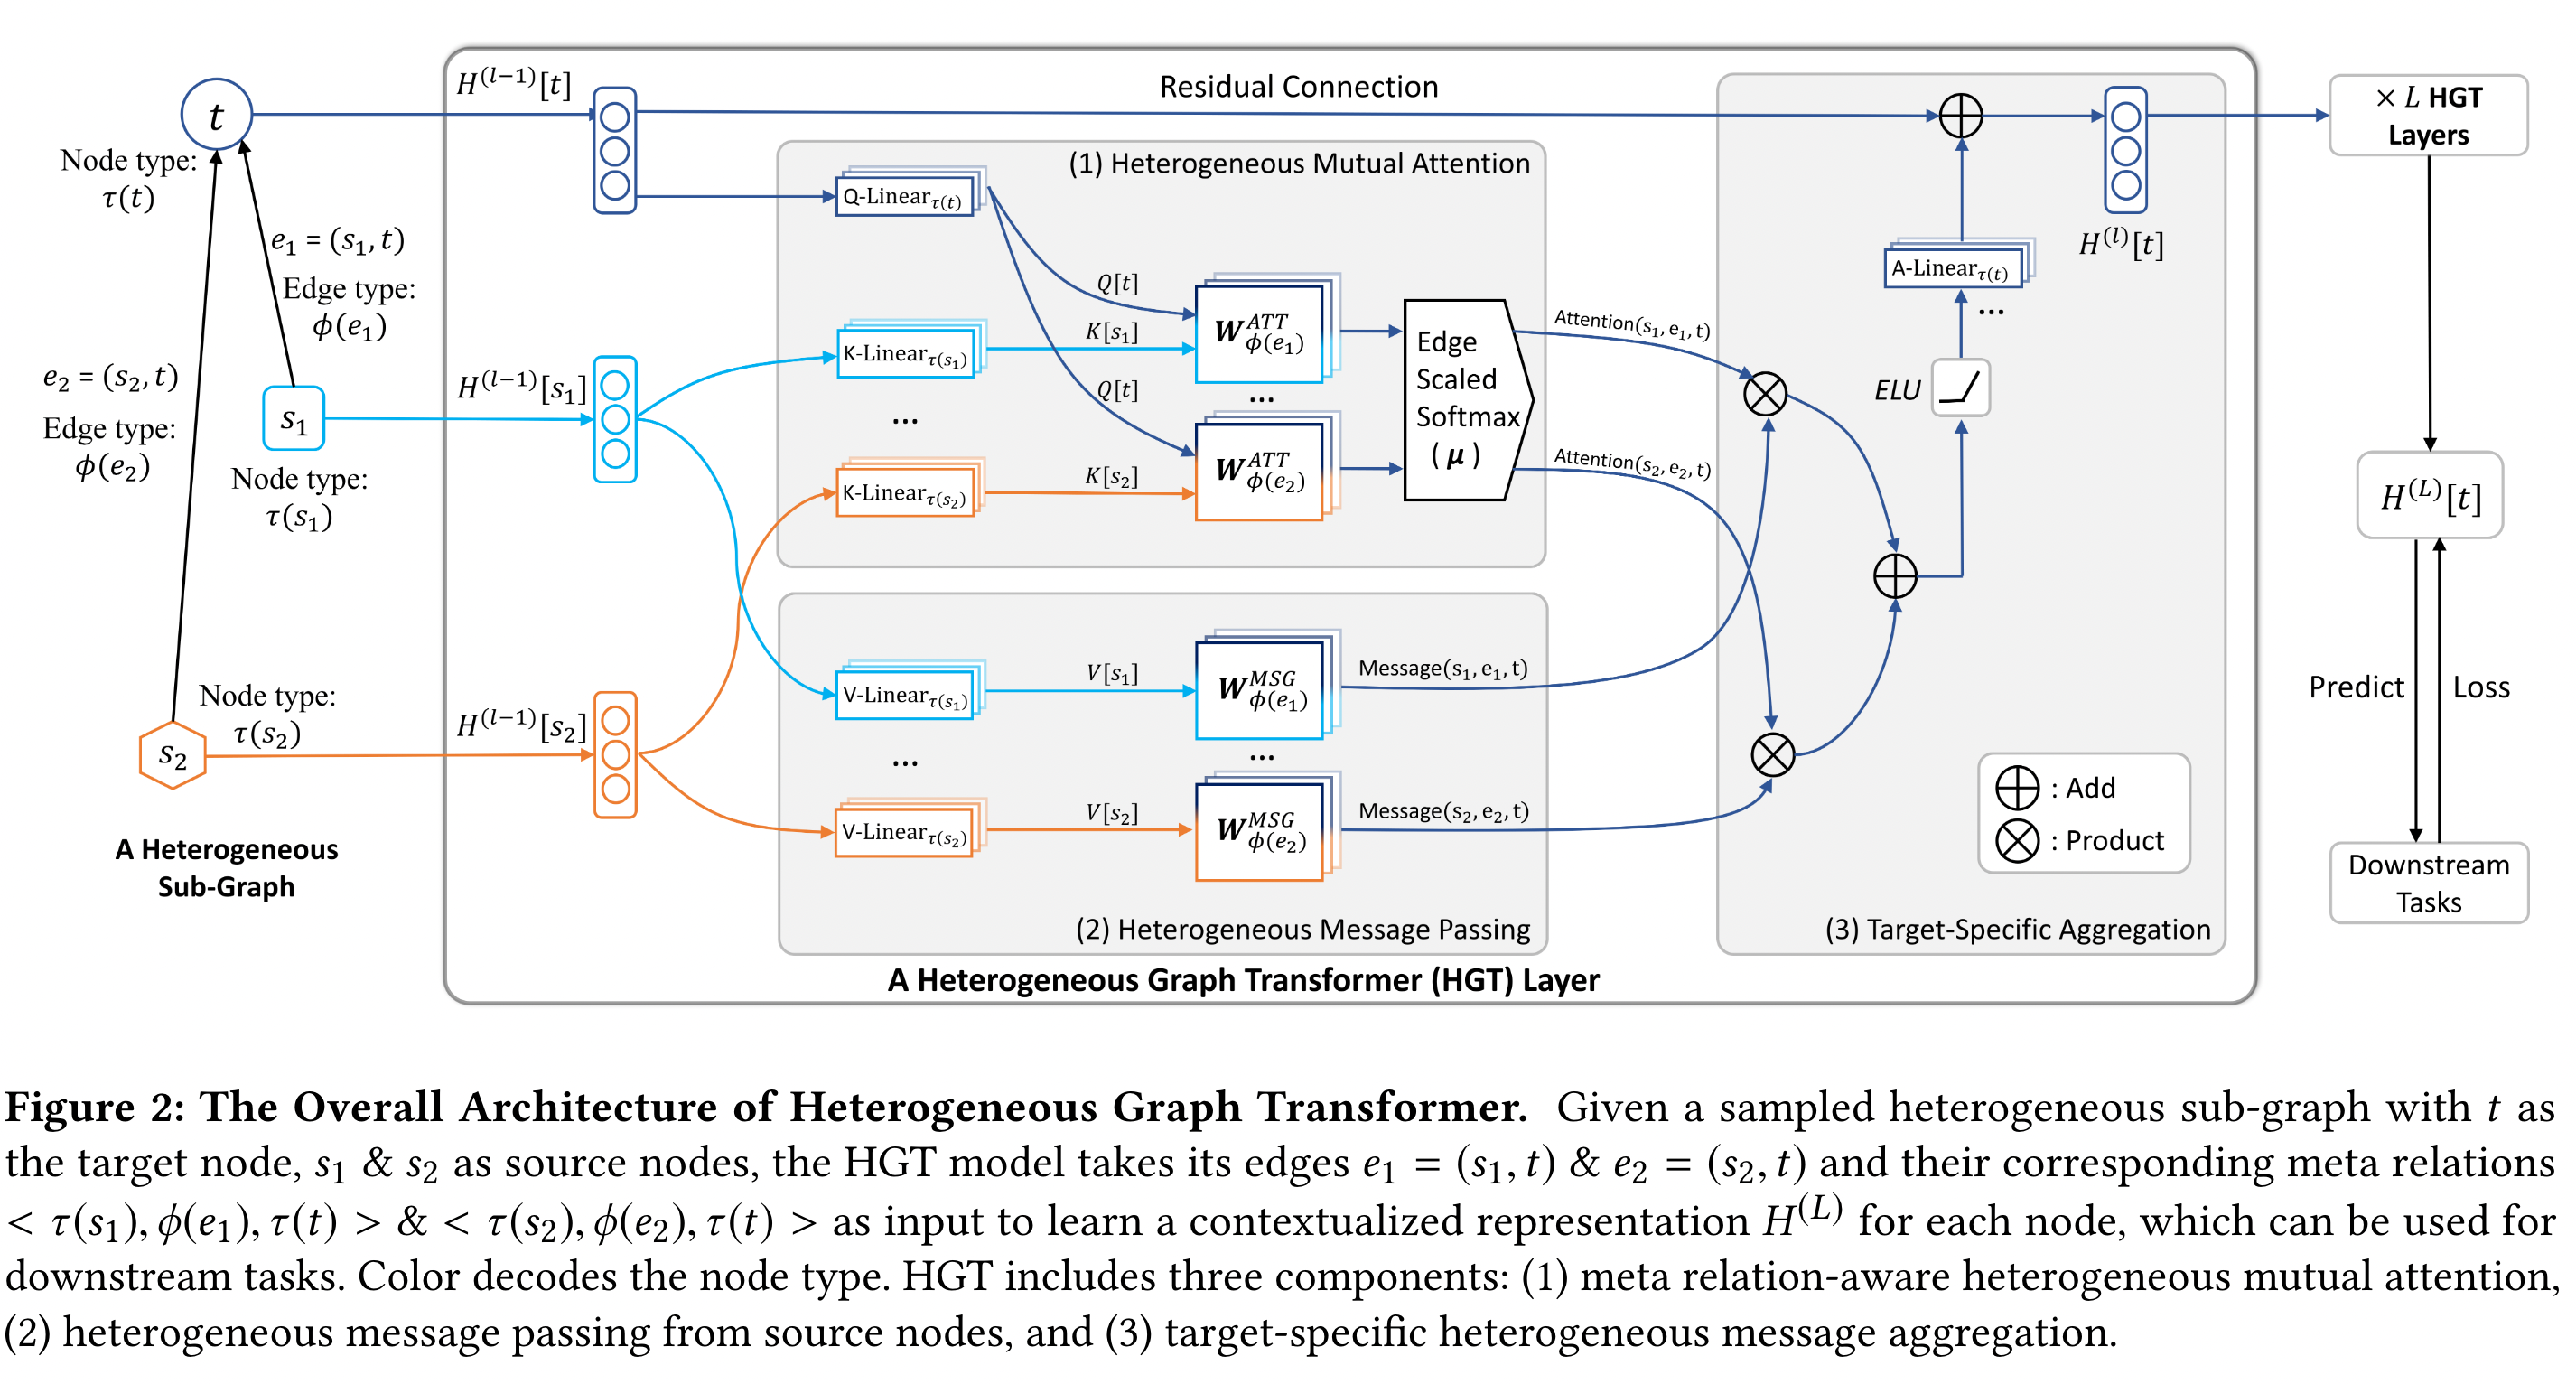
\includegraphics[width=.9\linewidth]{./p2.png}
\end{center}
\end{frame}

\begin{frame}[label={sec:org77e49dd}]{Heterogeneous Mutual Attention}
GAT:

\begin{center}
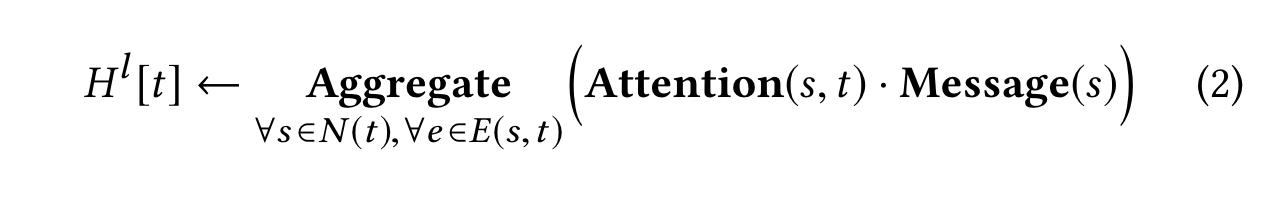
\includegraphics[width=10cm]{./p3-1.png}
\end{center}
\begin{center}
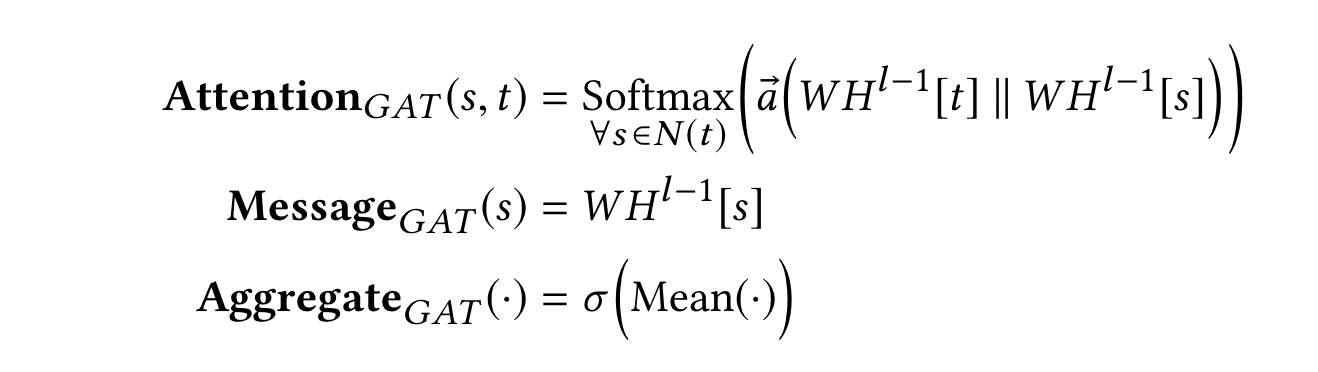
\includegraphics[width=10cm]{./p3-2.png}
\end{center}

\begin{description}
\item[{Attention}] Importance of each source node.
\item[{Message}] Extracts the message by using only the source node.
\item[{Aggregate}] Aggregate the neighborhood message by the attention weight.
\end{description}
\end{frame}

\begin{frame}[label={sec:org06bd389}]{Heterogeneous Mutual Attention}
Transformer:  \(W_q,W_k,W_v\)

HGT:
\begin{center}
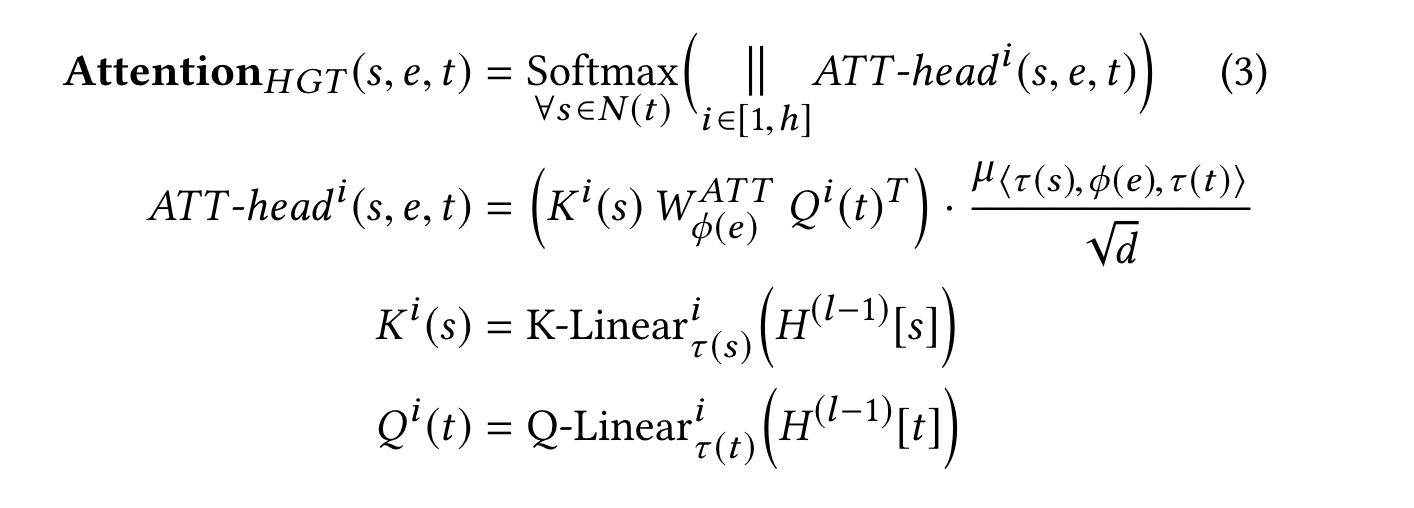
\includegraphics[width=10cm]{./p4.png}
\end{center}

\begin{itemize}
\item \(W^{ATT}_{\phi(e)}\)
\item \(\mu_{<\tau(s),\phi(e),\tau(t)>}\)
\end{itemize}
\end{frame}

\begin{frame}[label={sec:org3d00681}]{Message passing}
\begin{center}
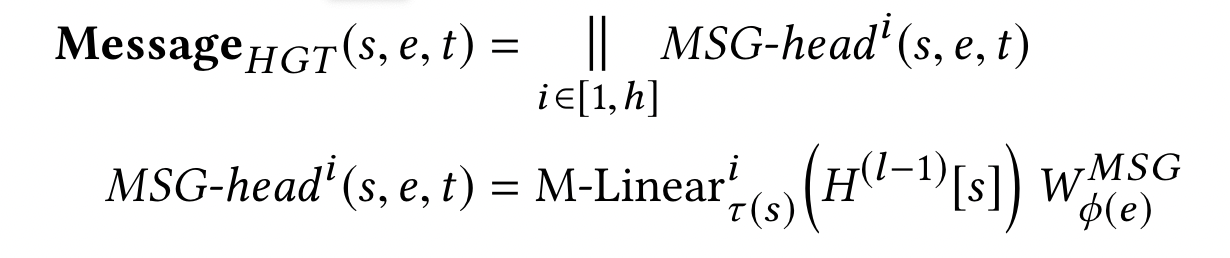
\includegraphics[width=.9\linewidth]{./p5.png}
\end{center}

\begin{itemize}
\item Edge dependent: \(W^{(MSG)} _{\tau(e)}\)
\item Incorporate the meta relations of edges into the message passing
process to alleviate the distribution differences of nodes and edges
of different types.
\end{itemize}
\end{frame}

\begin{frame}[label={sec:org155b484}]{Target-Specific Aggregation}
\begin{center}
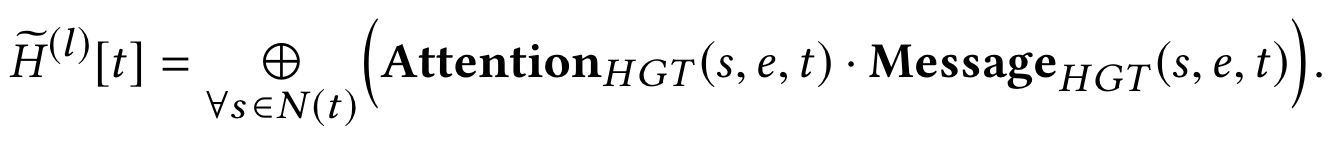
\includegraphics[width=10cm]{./p6.png}
\end{center}
\begin{center}
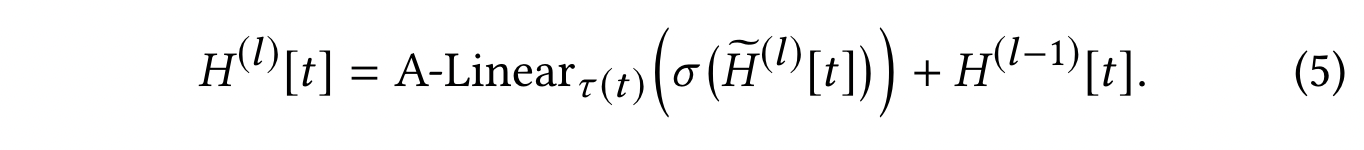
\includegraphics[width=10cm]{./p6-2.png}
\end{center}

\begin{itemize}
\item A-Linear\(_{\tau(t)}\) to map target node \(t\) to type specific
distribution and update the \(l\)-th HGT layers embedding.
\end{itemize}
\end{frame}

\begin{frame}[label={sec:org2d456c3}]{HGSampling}
\begin{center}
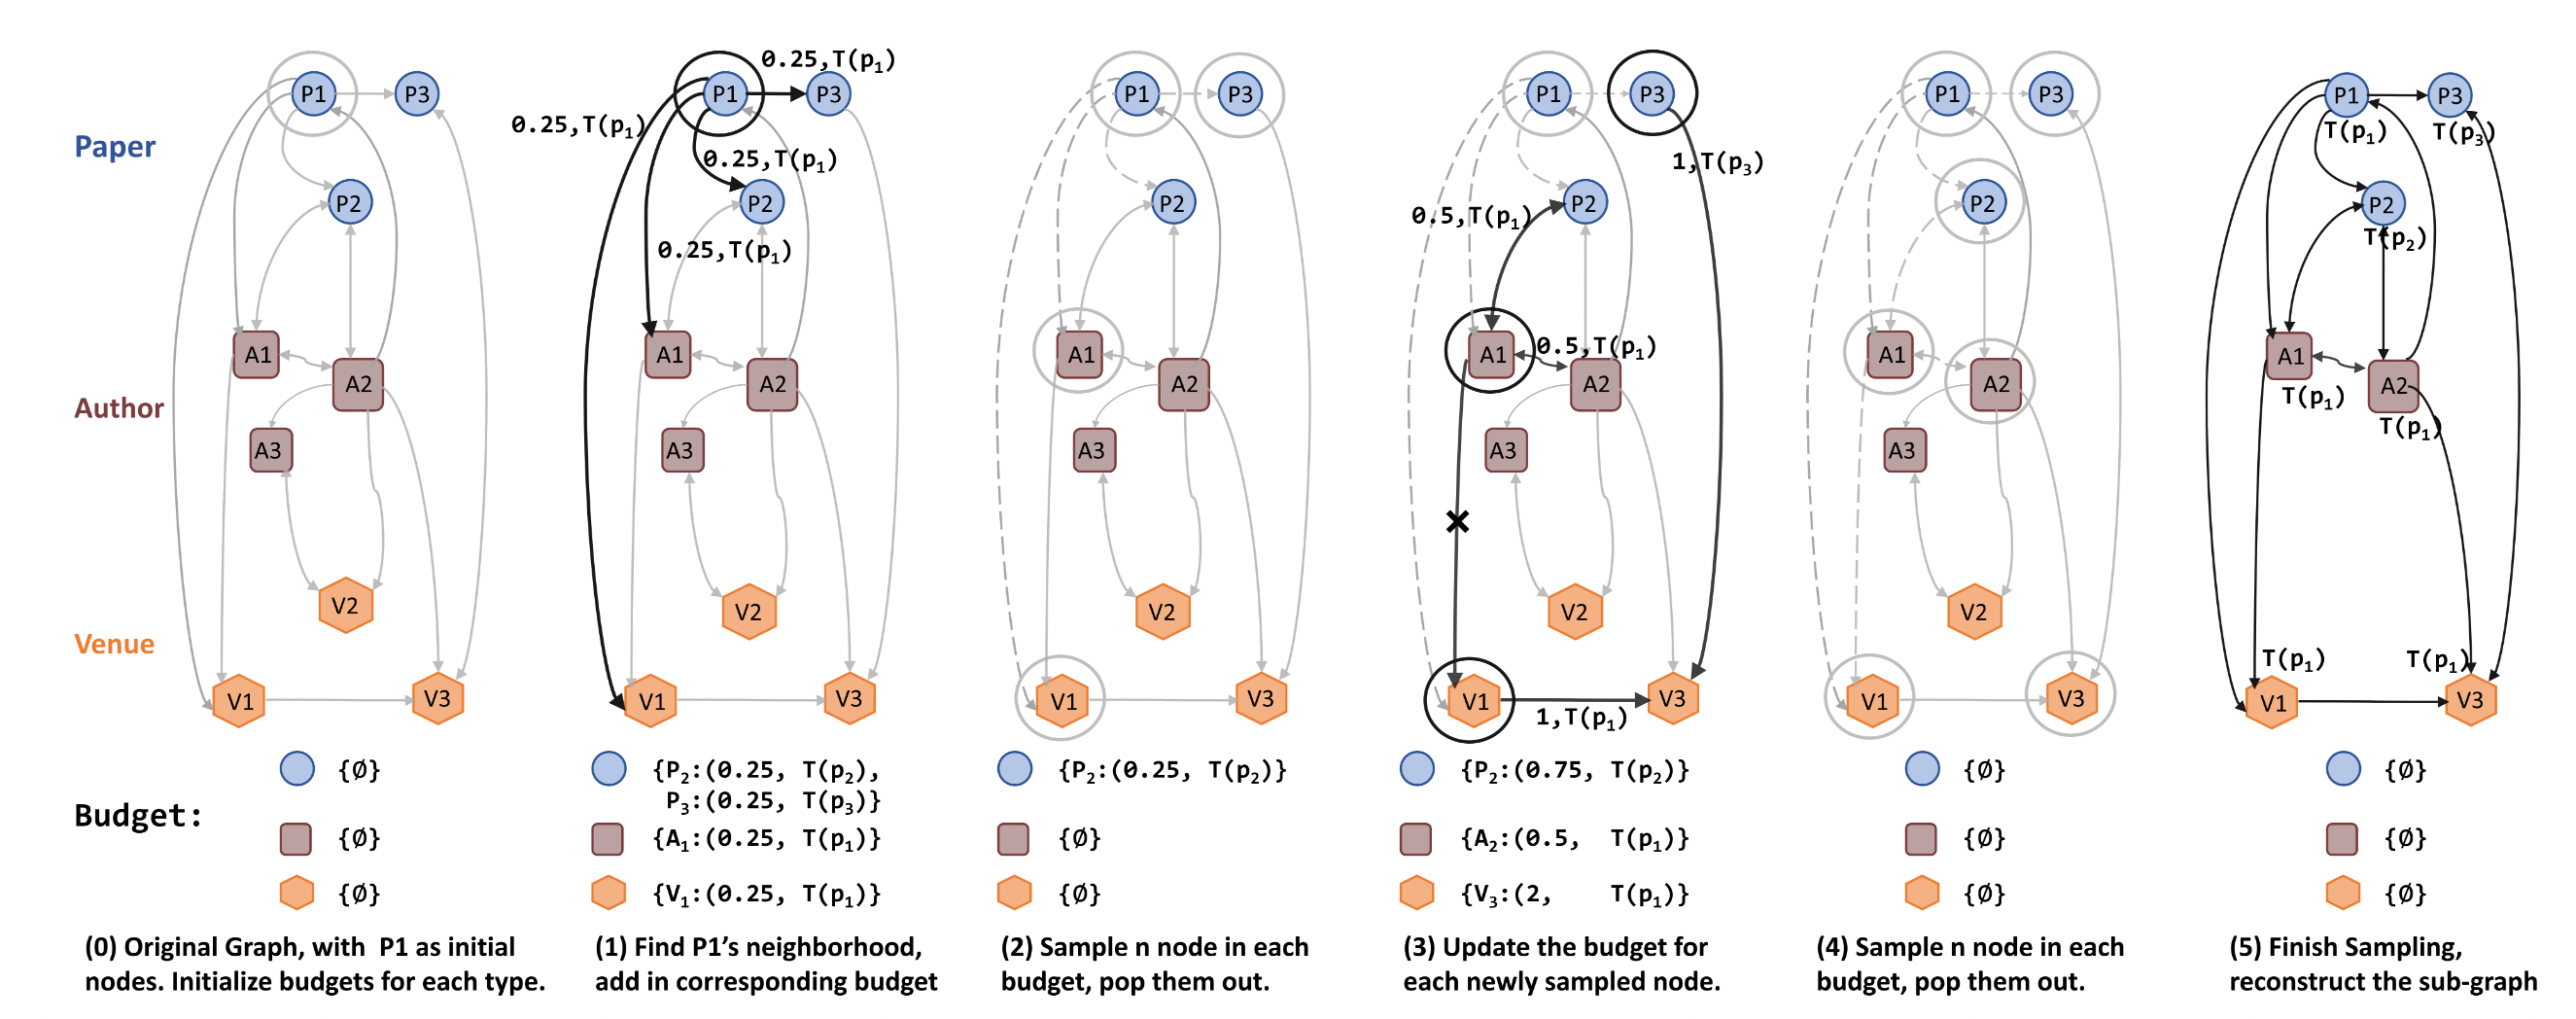
\includegraphics[width=.9\linewidth]{./p7.png}
\end{center}

\begin{itemize}
\item keep a similar number of nodes and edges for each type, and keep the
sampled sub-graph dense to minimize the information loss and reduce
the sample variance.
\end{itemize}
\end{frame}

\begin{frame}[label={sec:org1d74f83}]{Relative Temporal Encoding (RTE)}
\begin{center}
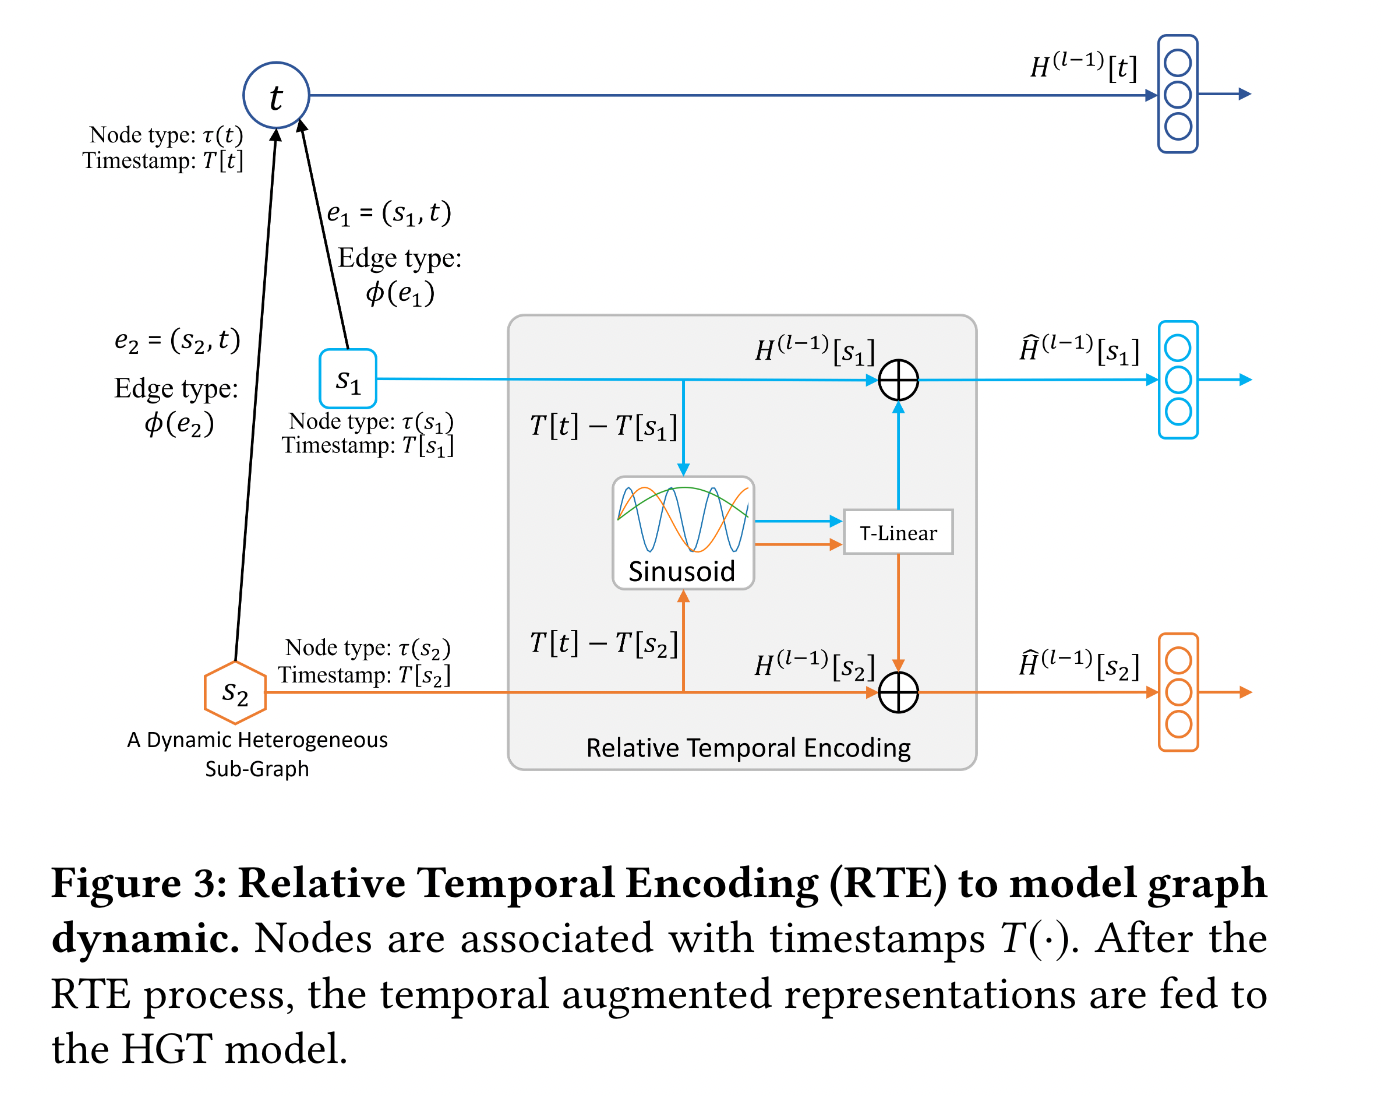
\includegraphics[width=10cm]{./p8.png}
\end{center}
\end{frame}

\begin{frame}[label={sec:org5640f02}]{Relative Temporal Encoding (RTE)}
\begin{center}
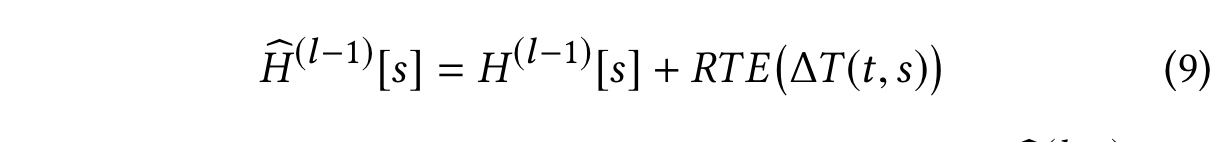
\includegraphics[width=.9\linewidth]{./p8-2.png}
\end{center}

\begin{itemize}
\item \(\Delta T(s, t) = T(s) - T(t)\)
\end{itemize}
\end{frame}

\section{Experiments}
\label{sec:orgb08a254}

\begin{frame}[label={sec:org4314065}]{OAG Data}
\begin{center}
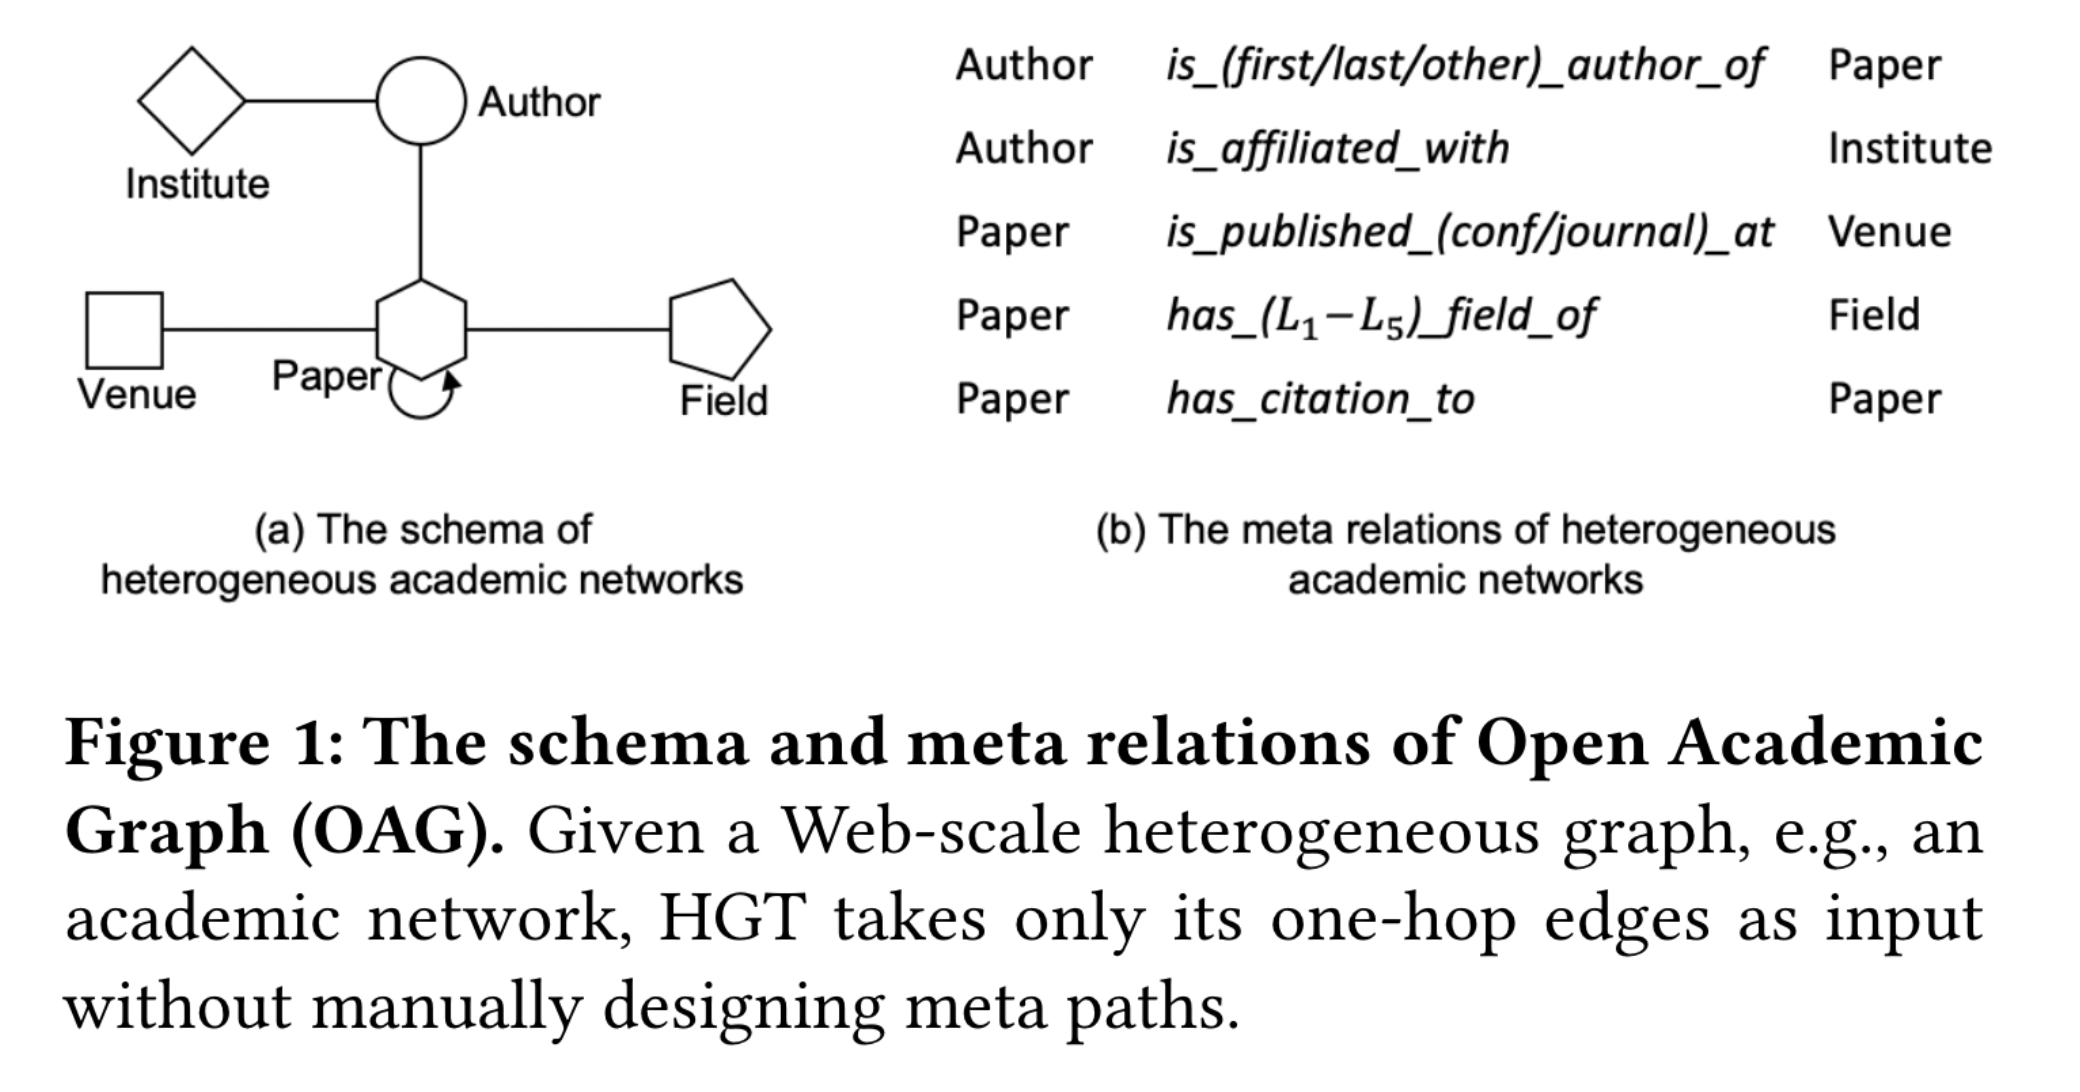
\includegraphics[width=.9\linewidth]{./p9.png}
\end{center}
\end{frame}

\begin{frame}[label={sec:orge41607b}]{OAG Data}
\begin{itemize}
\item OAG
\begin{itemize}
\item All
\item Computer Science (CS)
\item Medicine (Med)
\end{itemize}
\end{itemize}
\end{frame}

\begin{frame}[label={sec:org7d628d4}]{Baseline models}
\begin{itemize}
\item Graph Convolutional Networks (GCN)
\item Graph Attention Networks (GAT)
\item Relational Graph Convolutional Networks
\begin{itemize}
\item Keep a different weight for each relationship (edge).
\item \(h_{i}^{(l+1)}=\sigma\left(\sum_{r \in \mathcal{R}} \sum_{j \in\mathcal{N}_{i}^{r}} \frac{1}{c_{i, r}} W_{r}^{(l)}h_{j}^{(l)}+W_{0}^{(l)} h_{i}^{(l)}\right)\)
\end{itemize}
\item Heterogeneous Graph Neural Networks
\begin{itemize}
\item Adopt different BiLSTM for node type and neighbor information
\end{itemize}
\item Heterogeneous Graph Attention Networks (HAN)
\begin{itemize}
\item Hierarchical attentions to aggregate neighbor via meta-paths
\end{itemize}
\end{itemize}
\end{frame}

\begin{frame}[label={sec:org36febc0}]{Results}
\begin{center}
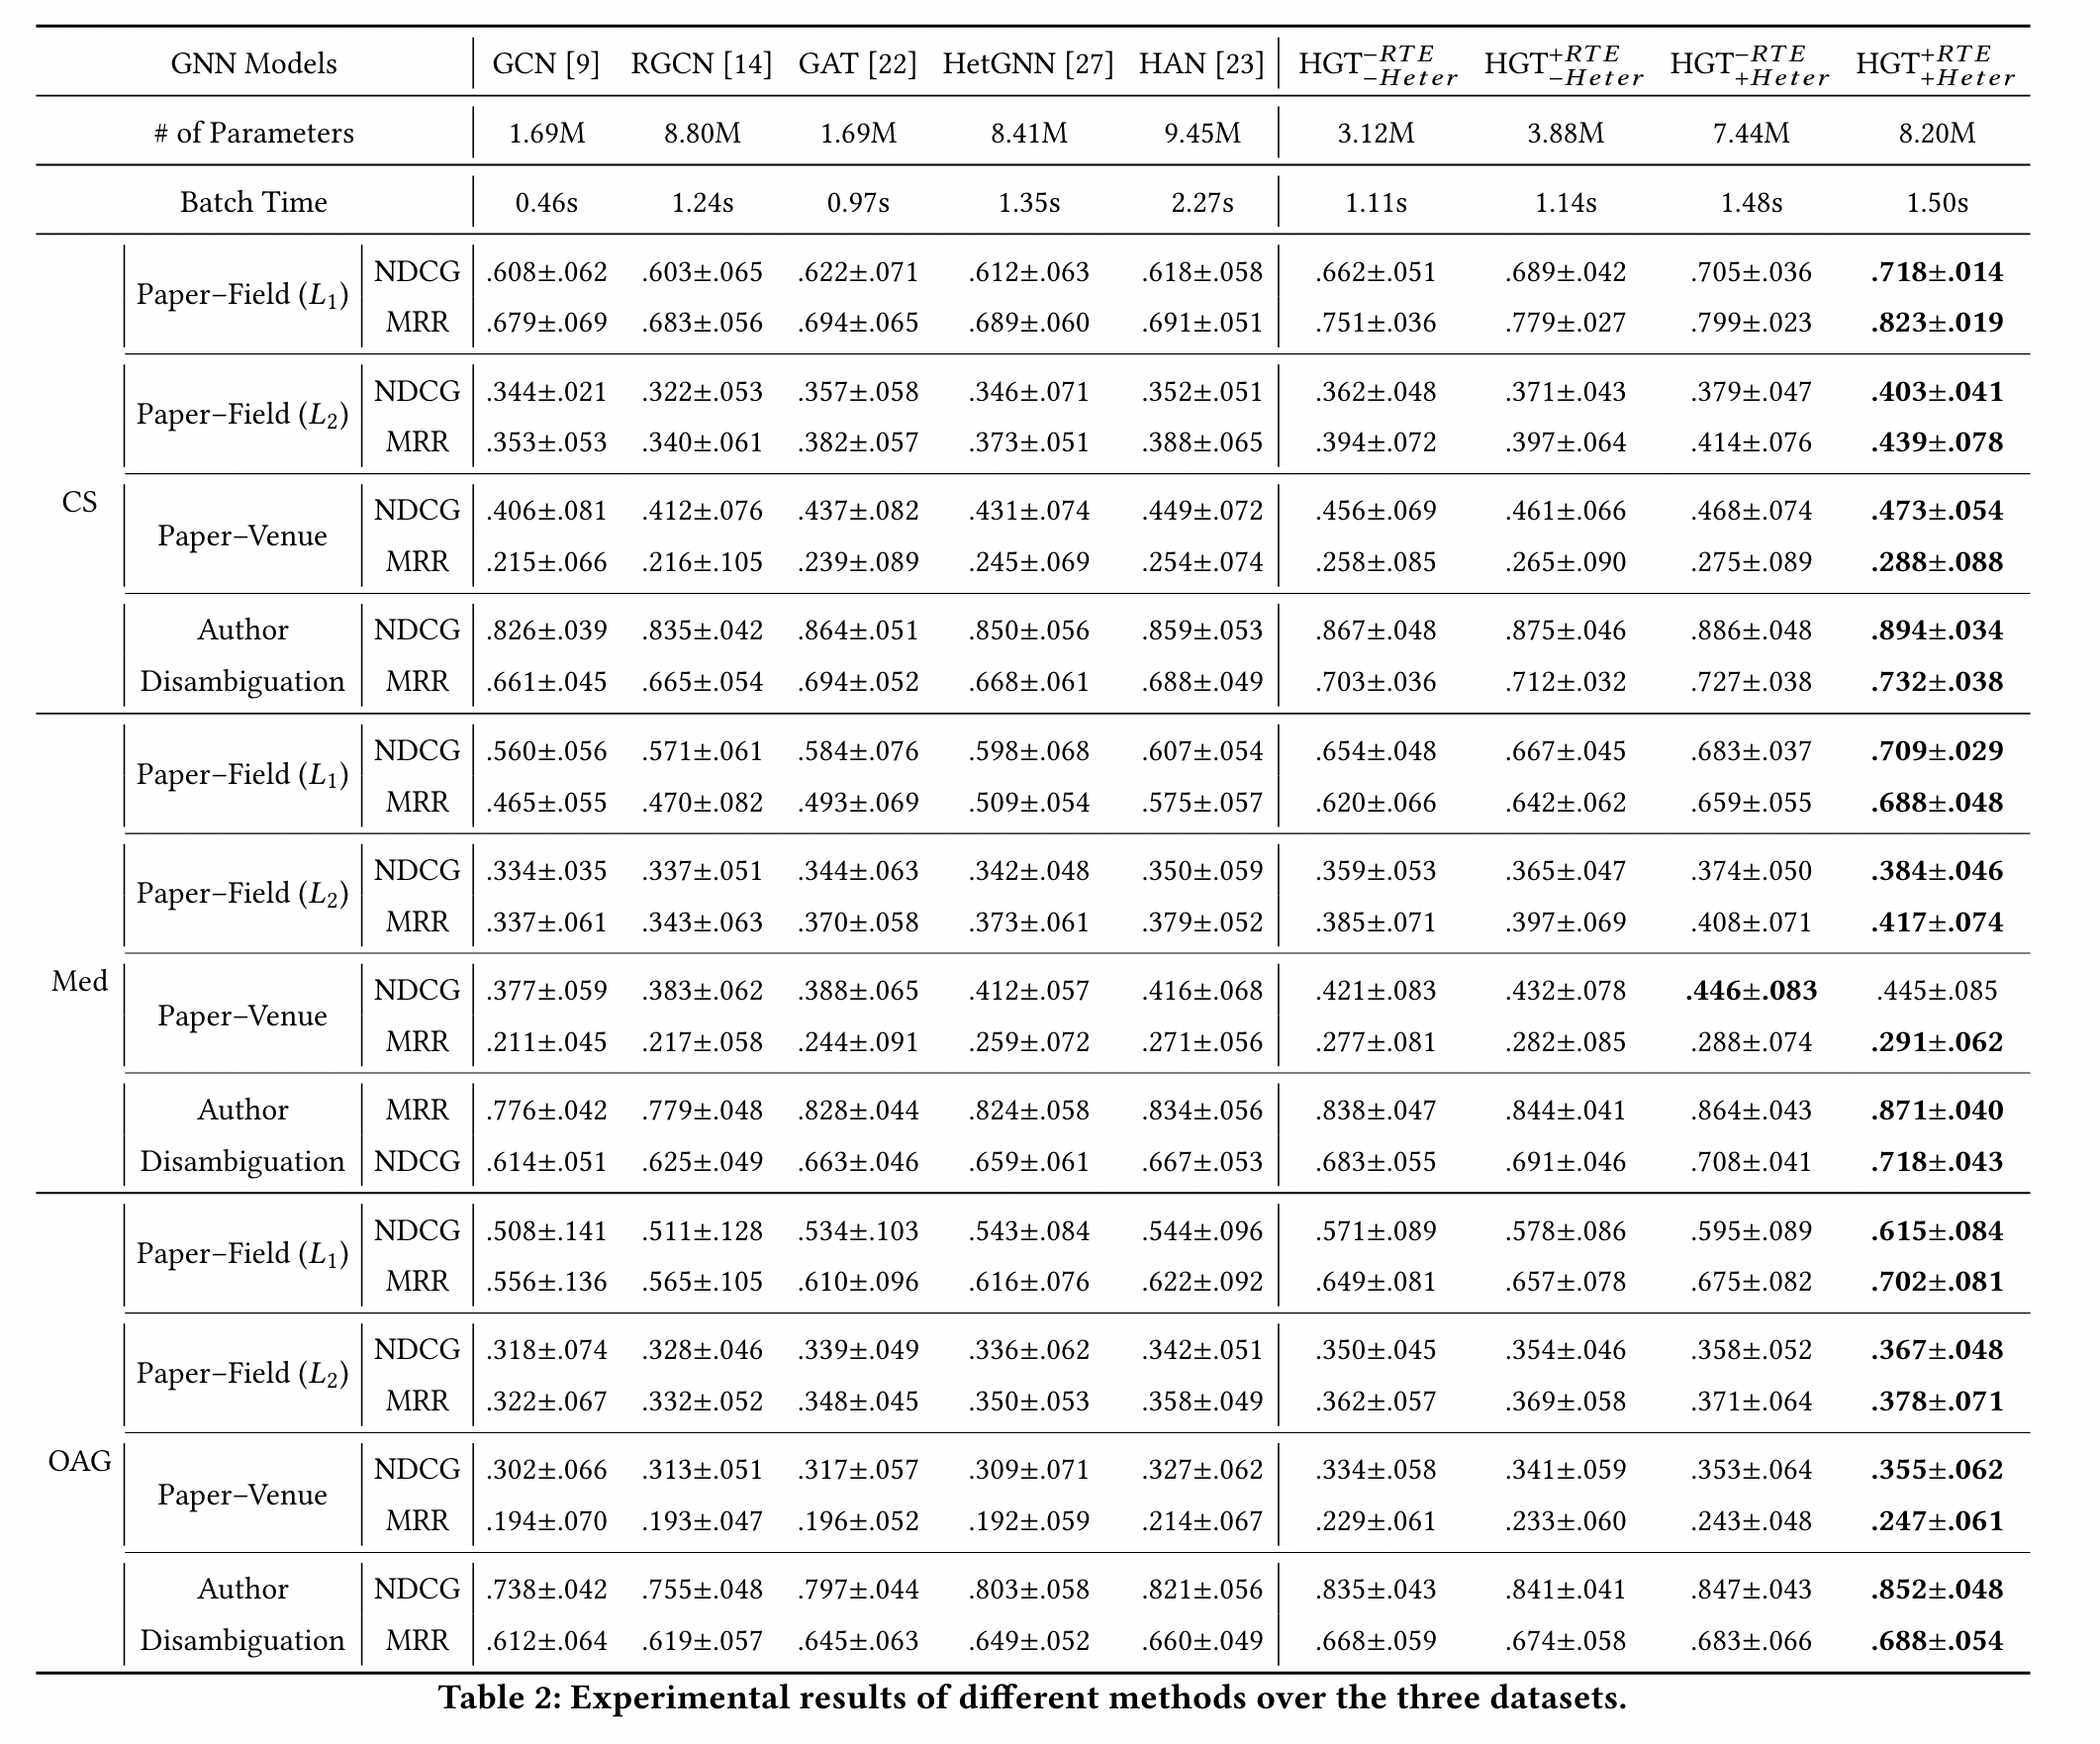
\includegraphics[height=8cm]{./p10.png}
\end{center}
\end{frame}

\section{Futures}
\label{sec:orga0fc50f}

\begin{frame}[label={sec:org7ffbf3a}]{Futures}
\begin{itemize}
\item Generate heterogeneous graphs
\begin{itemize}
\item predict new papers and title
\end{itemize}
\item Pre-train HGT to benefit tasks with scarce labels
\end{itemize}

---

\begin{itemize}
\item Downstream Tasks
\end{itemize}
\end{frame}
\end{document}